% !TeX root = ../notes.tex

\section{Introduction}
Queries involve multiple steps to be performed. All techniques obviously depend on the physical characteristic of hardware, however there are algorithms and data structures able to help making them faster.

Query optimization is specifically important since SQL-like languages are \textit{declarative}, hence do not specify the exact computation. Furthermore, the same query can be performed in \textbf{multiple ways} with different runtime, and choosing the correct one is not trivial (depending on size, indices and more).

For instance, looking at cardinality of joins can either cause a Cartesian product of a hundred or several thousands, depending on the order in which they are executed. Often the human-written sequential order of instructions is not the most efficient one.

\subsection{Query Processing}
\begin{wrapfigure}{R}{0.2\textwidth}
	\vspace{-35pt}
	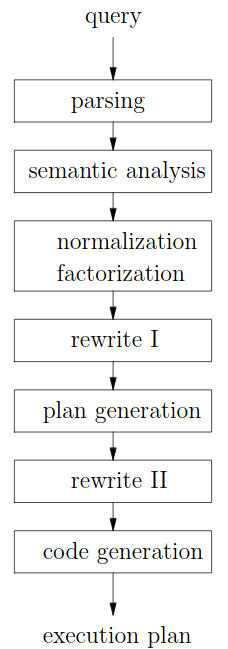
\includegraphics[width=0.2\textwidth]{runtime_system.png}
	\vspace{-100pt}
\end{wrapfigure}
Query processing consists in: 
\begin{enumerate}
	\item Taking a text query as input;
	\item Compiling and optimizing;
	\item Extract the execution plan;
	\item Executing the query.
\end{enumerate}
Roughly, it can be differentiated between \textbf{compile time} and \textbf{runtime system}. Most systems strongly separate those phases, for example using so-called prepared queries.
\begin{lstlisting}[language=SQL]
SELECT S.NAME
FROM STUDENTS S
WHERE S.ID = ?
\end{lstlisting}

Compilation takes time and limits the number of queries which can be ran in parallel. This kind of query can be executed over and over providing a value \texttt{Q1(123)} without the compilation overhead.

\textit{Embedded SQL} is another technique to optimize compilation time in the case of large periods of time between the two phases, combining data manipulation with low-level code. The programming language compiler takes care of the SQL part as well, optimizing it.

The embedded SQL statements are parsed by a preprocessor and replaced by host-language calls to a code library, and from the preprocessor is then compiled by the host compiler.

The steps executed in compile time in a general database environment are:
\begin{enumerate}
	\item \textbf{Parsing}, AST production (abstract syntax to understand the structure);
	\item \textbf{Schema lookup}, variable binding, type inference (semantic analysis \textbf{about} relations and columns, syntax check);
	\item \textbf{Normalization}, factorization (bringing the query in abstract form, avoiding computing the same thing twice, evaluating expressions);
	\item \textbf{Unnesting}, deriving predicates, resolution of views (the plan generator can finally construct a cost-based model);
	\item \textbf{Construction} of execution plan;
	\item \textbf{Review}, pushing joins and refining the plan in general;
	\item \textbf{Production} of imperative plan (code generation).
\end{enumerate}
Rewrite I involves steps 1-3, while 4 and 5 compose rewrite II.

Example (with views):
\begin{lstlisting}[language=SQL]
SELECT name, salary
FROM employee, department
WHERE dep = did
AND location = "Munich"
AND area = "Research"
\end{lstlisting}
The query goes through the first phase of semantic analysis, is normalized (the equivalences are pushed down, before applying AND) and then unnested. 

\begin{figure}[h]
	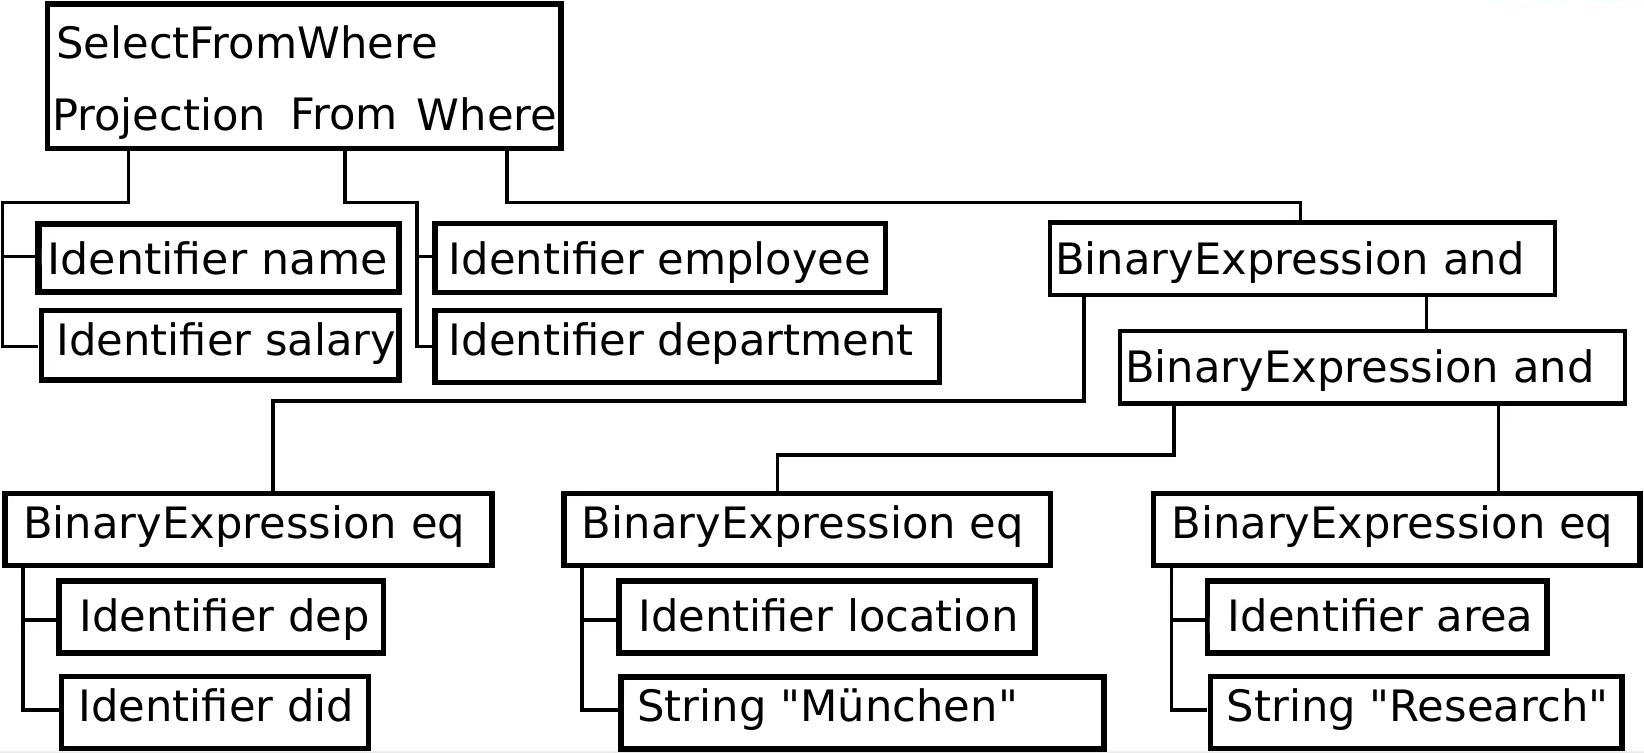
\includegraphics[scale=1.1]{query_plan.png}
	\centering
\end{figure}
Finally, the execution tree with \textbf{relational algebra} operators is built and polished, with the join operation on top and selects on nodes, reducing the amount of tuples to be joined. In other cases, such as regular expressions which are hard to evaluate, filtering can be done later.

The \textbf{executable plan} is a set of tuples containing variables or constants along and their type, with the main function loading query parameters, operations and allocated resources. 

Usually query planners are much more complicated and have practical difficulties: for instance, a long list of AND/OR predicates (machine-generated in the order of hundreds of thousands) can make the binary tree recursion crash due to insufficient space in the stack.

\subsection{Query Optimization}
Possible goals of query optimization include minimizing response time, resource consumption, time to first tuple (producing the first tuple as quick as possible, for instance with search results) or maximizing throughput. This can be expressed as a \textbf{cost function}: most systems aim to minimize response time, having resources as constraints.

\textbf{Algebraic optimization} is a branch using relational algebra to find the cheapest expression equivalent to the original. However, finding the cheapest is a \textbf{practically impossible problem}: it is hard to test for equivalence (numerical overflow, undecidable), the set of expressions is potentially huge and some algorithms are NP-hard (actual search space is limited and smaller than the potential one). 

There are ways to transform numerical expressions in algebraic ones, yet they might be expensive: calculus is faster to evaluate than algebra. 

Optimization approaches can be:
\begin{itemize}
	\item \textbf{Transformative}, taking an algebraic expression and iteratively making small changes, not efficient in practice;
	\item \textbf{Constructing}, starting from small expressions and joining them, obtaining larger sets, usually the preferred approach.
\end{itemize}

\subsection{Query Execution}
Query execution is the last step, the one \textbf{directly benefiting from optimization}. In reality, operators can perform extremely specialized operations, treating data as bags (sets with duplicates) or streams.

\subsubsection{Relational and physical algebra}
Relational algebra for query optimization includes the operators of \textbf{projection}, \textbf{selection} and \textbf{join}, plus some additional ones such as \textbf{mapping} and \textbf{grouping}.

However, this does not imply an implementation, which can have a great impact, hence less abstract operators are needed due to \textbf{stream} nature of data (and not sets):
\begin{itemize}
	\item \textbf{Sort}, according to criteria;
	\item \textbf{Temp}, which \textit{materializes the input stream} making further reads cheaper and releasing memory afterwards;
	\item \textbf{Ship}, sends the input stream to a different host (for distributed computing).
\end{itemize}

Furthermore, there are different kind of joins having different characteristics:
\begin{itemize}
	\item \textbf{Nested Loop Join}, the textbook implementation which is very slow (quadratic) but supports all predicates;
	\item \textbf{Blockwise Nested Loop Join}, reading chunks of the first column in memory and then the second one once (requires memory, can be improved using hashing). The left side is read $\frac{\abs{L}}{\abs{M}}$ times, which asymptotically is the same as above but in practice \textit{much faster};
	\item \textbf{Sort Merge Join}, scanning each column only once, but requiring sorted input ($O(n\log n)$ plus linear runtime assuming no duplicates on at least one side);
	\item \textbf{Hybrid Hash Join}, partitioning columns and joining them in memory (linear time, but working only for equi-joins).
\end{itemize}

Hash Join is usually the fastest, but with very large amount of data sorting might be more efficient. Nested Loop Join works well when one of the sides has only one tuple.

Other operators also have different implementations, such as aggregation sorting and hashing, whose speed depends on the algorithm (quick sort, heap sort etc.) and can rely or not on memory.

Physical algebra is hence the output of the query optimizer, since it fixes the exact execution runtime and does not stop to the general approach like relational algebra. It mainly helps to select which operator to use before running the query, so that optimization leads to more efficient plans.

